\scanpage{75}
\mspage{74}

\margin{\handwritten{\figure{\begin{tikzpicture}[x=1cm,y=1cm]\draw[thin] (0,0)--(.45,.7);\end{tikzpicture}}On a un hom (une fois choisi $\bar{k}$ ; d'où une réalisation $\deleted{\unsure{G|C}}'$  de lien $\underline{\pi}_p(k)$) $\pi_1(k)_K\longrightarrowG'(K)$ d'où un foncteur $(\text{torseurs sous }\pi_1(k)_K)\longrightarrow\text{torseurs sous }G'$ et on prend l'image du torseur sous $\pi_1(k)_K$, défini en interprétant $\pi_1(k)$ comme Galois de l'extension non ramifiée \unsure{universelle|univers.} de $K$.}}
pro-fini ``abstrait'' $\handwritten{\pi}_1(k)$, mais on se convainc facilement qu'elles\deleted{et} sont contenues dans la donnée de ce groupe, $+$ son opération sur la clôture algébrique $\handwritten{\bar{K}}$ de $K$ (ou simplement, sur sa clôture non ramifiée .sur $W$ ...)\handwritten{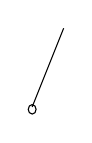
\begin{tikzpicture}[baseline=0cm,x=1cm,y=1cm]\draw[thin] (0,-.5)--(.4,.5);\draw[thin] (0,-.53) ellipse (.05 and .06);\end{tikzpicture}}. - Il resterait enfin à déterminer la structure d'effectivité dans la catégorie $\mathrm{Fcriso}(k)$ dé\deleted{\unsure{terminé}}\handwritten{\unsure{terminé}}e par la récette précédente\deleted{\unsure{.} la suggestion naturelle est que $\mathrm{Fcriso}^{\handwritten{+}}(k)$ est engendré par les images de $\mathrm{Fcriso}^{\handwritten{+}}$} Or il est immédiat que l'effectivité d'un F-isoc\unsure{\.{r}|r}\unsure{\.{r}|i}stal est invariante par changement de base, en particulier par le changement de base $k\handwritten{\longrightarrow\bar{k}}$, ce qui ramène au cas d'un $k$ algébriquement clos, ou encore au cas de $\underline{F}_p$ . \deleted{En}\handwritten{Dans} \deleted{termes de} la terminologie introduite plus bas, on trouvera donc que les $\unsure{\mathbb{F}|\rlap{$G$}F|F|E}$-isocristaux effectifs sont ceux qui sont \uline{à pente} $\handwritten{\geq}0$ (i.e. dont toutes les composantes isopentiques \deleted{sont} non nulles sont de pente $\handwritten{>}\ 0$).

\handwritten{8.} Il reste donc à étudier la gerbe $\underline{G}(\underline{F}_p)$, avec s\unsure{\rlap{o}a|a|o}\deleted{n} \deleted{foncteur fibre,} section canonique sur $\underline{Q}_p$, sa structure d'extension, et sa structure d'effectivité.

\margin{\handwritten{\figure{\begin{tikzpicture}\draw (0,0) -- (0.65,0.04) -- (0.65,0.8) -- (1.1,0.8);\end{tikzpicture}}}}
\inserted{\handwritten{8.1.}}\handwritten{\begin{tikzpicture}[baseline=0cm,x=1cm,y=1cm]\draw[gray,thin] (0,-.35)..controls (-.13,-.1) and (.05,.04)..(.1,.1)--(.8,.08)..controls (1,.08) and (1.1,.15)..(1.08,.25);\end{tikzpicture}} Tout d'abord, la donnée du foncteur fibre canonique permet d'identifier $\underline{G}(\underline{F}_p)$ à la gerbe\handwritten{\begin{tikzpicture}[baseline=0cm,x=1cm,y=1cm]\draw[gray,thin] (0,-.35)--(.27,.45);\end{tikzpicture}}triviale définie par le lien \inserted{\handwritten{$G$}}\handwritten{\begin{tikzpicture}[baseline=0cm,x=1cm,y=1cm]\draw[gray,thin] (0,-.35)--(.27,.45);\end{tikzpicture}} de cette gerbe. Comme $\mathrm{Fcriso}(F_p)$ avec son foncteur fibre s'identifie à la catégorie des automorphismesde\inserted{$F_E$}\handwritten{\begin{tikzpicture}[baseline=0cm,x=1cm,y=1cm]\draw[gray,thin] (0,-.35)--(.27,.45);\end{tikzpicture}} vectoriels de dimension finie\inserted{$E$}\handwritten{\begin{tikzpicture}[baseline=0cm,x=1cm,y=1cm]\draw[gray,thin] (0,-.35)--(.27,.45);\end{tikzpicture}} sur $\underline{Q}_p$, avec le foncteur ``oubli de $F_E$ '', on voit que le lien de la gerbe est l'enveloppe $\underline{Q}_p$-\inserted{pro}\handwritten{\begin{tikzpicture}[baseline=0cm,x=1cm,y=1cm]\draw[gray,thin] (0,-.3)..controls (-.08,-.12) and (.13,.1)..(.25,.08)..controls (.65,.01) and (1,.14)..(1.12,.45);\end{tikzpicture}}algébrique de groupe discret $\underline{Z}$ . Soit $G$ ce groupe affine sur $\underline{Q}_p$ . I\begin{tikzpicture}[baseline=(l.base),x=1cm,y=1cm]\node[inner sep=0pt] (l) {l};\draw[thin] (-.17,.55)--(.13,.55)--(.13,.62);\draw[thin] (-.05,.55)--(-.05,.61);\draw[thin] (-.17,-.12)..controls (.06,-.07) and (.04,-.13)..(.01,-.4);\end{tikzpicture} est évidemment commutatif, donc produit d'un groupe vectoriel $G_u$ par un groupe de t.m. $G_{\deleted{\unsure{m}}r}$ .
\margin{\handwritten{\unsure{réf|cf}\figure{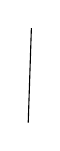
\begin{tikzpicture}\draw (0,0) -- (0.04,1.2);\end{tikzpicture}}}}
Ce dernier est l'enveloppe \inserted{de type}\handwritten{\begin{tikzpicture}[baseline=0cm,x=1cm,y=1cm]\draw[gray,thin] (0,-.2)..controls (0,.08) and (.27,.06)..(.4,.07)--(1.6,.1)..controls (1.8,.12) and (1.8,.13)..(1.74,.33);\end{tikzpicture}} multiplicati\deleted{ve}\handwritten{f} du groupe $\underline{Z}$, et il s'ensuit aussitôt que c'est le groupe de t.m. dont le groupe des caractères sur $\handwritten{\bar{\underline{Q}}}_p$ est donné par
\[
\handwritten{\Gamma}=\handwritten{\bar{\underline{Q}}}_p^{\handwritten{*}}\ ,
\]
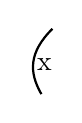
\begin{tikzpicture}[baseline=(x.base),x=1cm,y=1cm]\node[inner sep=0pt] (x) {\unsure{x}};\draw[thick] (.1,.45)..controls (-.2,.15) and (-.2,-.1)..(-.04,-.38);\end{tikzpicture}isomorph\unsure{\rlap{o}i|i|o}sme compatible avec l'action de $\operatorname{Gal}(\handwritten{\bar{\underline{Q}}}_p/\underline{Q}_p)$ ). D'autre
